%!TEX program = xelatex
\documentclass{beamer}

\usetheme{Execushares}


\title{Simulation of a \\ \vspace{.4cm} tennis ball throwing machine}
\subtitle{A competition announced by the E-10 Simulation GmbH }
\author{Lars Schiller}
\date{\today}

\setcounter{showSlideNumbers}{1}
  
\begin{document}
	\setcounter{showProgressBar}{0}
	\setcounter{showSlideNumbers}{0}

	\frame{\titlepage}

	\setcounter{framenumber}{0}
	\setcounter{showProgressBar}{1}
	\setcounter{showSlideNumbers}{1}
	
	
	
	%% Begin
	\section{Introduction}
		\begin{frame}
			\frametitle{Task description}
			
			\begin{center}
			\begin{tikzpicture}[scale = .55]
			%% Axis
			%\draw[help lines,step = 2] (0,0)grid (15,9);
			\draw[help lines,dotted] (-2,1)-|(0,-1);
			\draw[help lines,dotted] (-2,0)-|(14,-1);
			
			%% Some values
			\def\scale{.32}
			\def\yO{7.2*\scale}
			\def\xO{14.53*\scale};
			\def\vw{-10*\scale};
			\def\k{0.08}
			
			\pgfmathsetmacro{\vrel}{sqrt((\xO-\vw)^2 + (\yO)^2)}
			\pgfmathsetmacro{\Fx}{\k*\vrel*(\xO-\vw)}
			\pgfmathsetmacro{\Fy}{\k*\vrel*(\yO)}
			\pgfmathsetmacro{\vabs}{sqrt((\xO)^2 + (\yO)^2)}
			\pgfmathsetmacro{\Fabs}{sqrt((\Fx)^2 + (\Fy)^2)}
			
			
			
			\draw[->] (0,-1)--(15,-1)node[right=.1cm]{$y_1$};
			\draw[->] (-2,0)--(-2,1.5)node[left=.1cm]{$y_2$};
			\foreach \x in {0,14}{\draw (\x,-1-.1)node[below]{\x}--(\x,-1+.1);}
			\foreach \y in {0,1}{\draw (-2-.1,\y)node[left]{\y}--(-2+.1,\y);}
			
			%% Ball
			\draw[fill=yellow] (0,1)circle(.4);
			\draw[very thin] (0,1)++(180+45:.5)--++(180+45:.3)node[below]{$m$};
			
			%% Points
			\def\w{.3}
			\draw [thick] (0,1)+(-45:\w)--+(135:\w) +(225:\w)--+(45:\w);
			\path (0,1)++(80:4) node[above,align = center,fill = ExecusharesWhite](A){Position of the \\ throwing machine: $\boldsymbol{y}_a$};
			\draw[very thin] (0,1)--(A);
			\draw [thick] (14,0)+(-45:\w)--+(135:\w) +(225:\w)--+(45:\w);
			\path (14,0) node[above=.2cm,align = center,fill=ExecusharesWhite]{Position of the \\ tennis ball \\ after 1.5 sec: $\boldsymbol{y}_b$};
			%% Trajectory we are looking for
			\pgfmathsetmacro{\a}{atan((\yO)/(\xO))}
			\path (0,1)coordinate(A);
			\draw[dotted,blue,thick] (A)to[out=\a,in=110](14,0)coordinate(B); 
			\draw[blue,thick,->] (A)--++(\a:\vabs)node[midway,above,sloped,rectangle,fill=ExecusharesWhite]{$\dot{\boldsymbol{y}}(0) =\,?$};
			
			\draw[blue,thick,dashed,->] (A)--++(\xO,0)node[midway,below]{$\dot{y_1}(0)$};
			\draw[blue,thick,dashed,->] (\xO,1)--++(0,\yO)node[near start,right]{$\dot{y_2}(0)$};
			
			
			%% Given elements
			\draw[->] (\xO-2*\vw+.5,1)--++(\vw,0)node[above,midway]{$v_w$};
			
			
			%% Elements were are looking for
			\draw[thick,red,-stealth] (0,3.5)--++(0,-2)node[right,midway]{$\boldsymbol{F}_g$};
			
			\draw[->,dashed,red] (A)++(0,-.1)--++(\xO-\vw,0)coordinate(X)node[midway,below]{$v_{rel1}(0)$};
			\draw[->,dashed,red] (A)++(\xO-\vw,0)--++(0,\yO)coordinate(X)node[midway,right]{$v_{rel2}(0)$};
			\draw[->,thick,red] (A)--(X)node[midway,below,sloped]{$\boldsymbol{v}_{rel}(0)$};
			
			\pgfmathsetmacro{\a}{atan((\yO)/(\xO-\vw))}
			\draw[thick,stealth-,red] (A)++(\a:\vrel+.5)coordinate(Fi)--++(\a:\Fabs)coordinate(F)node[midway,above,sloped]{$\boldsymbol{F}_w$};
			\draw[dashed,red,-stealth] (F)--++(0,-\Fy)coordinate(X)node[right,midway]{$F_{w2}$};
			\draw[dashed,red,-stealth] (X)--++(-\Fx,0)node[below,midway]{$F_{w1}$};			
			\end{tikzpicture}
			\end{center}
		
					
%			\begin{footnotesize}					
%			\begin{center}
%			\begin{tabular}{cc|cc|cccc|c}
%			$y_a$ & $y_b$  & $g$ & $v_w$ & $\rho_T$ & $\rho_L$ & $c_w$ & $r$ & $t_f$\\ \hline
%			(0,1) & (14,0) & 9.81$\frac{\textnormal{m}}{\textnormal{s}^2}$ & -10$\frac{\textnormal{m}}{\textnormal{s}}$ & $408\frac{\textnormal{kg}}{\textnormal{m}^3}$ & 1.225$\frac{\textnormal{kg}}{\textnormal{m}^3}$ & 0.47 & 34\,mm & 1.5\,s \\
%			\end{tabular}
%			\end{center}	
%			\end{footnotesize}	
		\begin{itemize}		
			\item We are looking for $\boldsymbol{\eta} := [\dot{y}_1(0)~~ \dot{y}_2(0)]^T$, the dropping velocity of the ball.		
		\end{itemize}
					
		
		
		\end{frame}

		\begin{frame}
			\frametitle{Mathematical model}
					~	
			 
			By defining $y_3 = \dot{y}_1$, $y_4 = \dot{y}_2$ and the state vector $\boldsymbol{y} = [y_1~~ y_2~~ y_3~~ y_4]^T$ we can set up a system of 1st order (non linear) differential equations:
			
			\begin{equation}
			\dot{\boldsymbol{y}}
			:=  f(\boldsymbol{y}) = 
			\begin{bmatrix}
			y_3 \\ y_4 \\
			-\frac{k}{m}|v_{rel}|\left(y_3-v_w\right)\\
			-\frac{k}{m}|v_{rel}|{y_4} - g
			\end{bmatrix},
			\label{eq:1stode}
			\end{equation}	
			with $|v_{rel}| = \sqrt{\left( \dot{y}_1 -v_w \right)^2 + \dot{y}_2^2}$.		
			
			
		 	Set up the Residual function: 
		 	\begin{equation}
		 	F(\boldsymbol{\eta}) := \boldsymbol{y}_\eta(t_f)-\boldsymbol{y}_b = 0,
		 	\label{eq:residualfun}
		 	\end{equation}
		 	 where $\boldsymbol{y}_\eta(t_f)$ is the solution of the initial value problem given in eq.~\ref{eq:1stode} with the initial condition $\boldsymbol{y}_0 = [\boldsymbol{y}_a ~~ \boldsymbol{\eta}]^T$ evaluated at $t = 1.5$.
			
			
		\end{frame}

	\section{Choice of suitable solvers}
		\begin{frame}
			\frametitle{Choice of suitable solvers}
			\begin{itemize}
			\item We need a method to find the zero of the residual function $F$ given in eq.~\ref{eq:residualfun}:
			\item The \textit{Newton}-method
				\begin{itemize}
					\item calculates the Jacobian of $F$ in each iteration step,
					\item needs $n+1$ evaluations of $F$ per step.
				\end{itemize}
			\item The \textit{Broyden}-method
				\begin{itemize}
					\item gets along with an approximation of the Jacobian,
					\item needs only $1$ evaluation of $F$ per step.
				\end{itemize}
			\item For more detailed information look up in the technical report.
			\end{itemize}
		\end{frame}


	\section{Evaluation of the results}
		\begin{frame}
			\frametitle{Evaluation of the results}
			

			\begin{tikzpicture}[remember picture,overlay]
				\path (current page.east)++(0,-1.7cm)node [opacity=0.2,left] {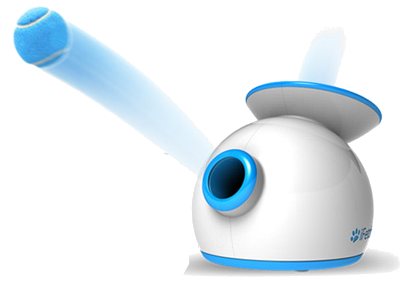
\includegraphics[width=8cm]{background_mirr.png}};
			\end{tikzpicture}			
			
			\begin{itemize}
				\item \textit{Newton} converges a bit faster,
				\item \textit{Broyden} needs less function evaluations and computational time.
				\item Therefore its reasonable to prefer the \textit{Broyden}-method.
			\end{itemize}
			
			\begin{center}
			\begin{tabular}{c|ccc}
			method & iteration steps & total evals of $f$ & comp. time [sec]\\
			\hline
			\textit{Newton} & 3 & 1010 & 0.0444 \\
			\textit{Broyden} & 4 & 509 & 0.0238 \\
			
			\end{tabular}
			\end{center}
			
			
		\end{frame}

\end{document}